\documentclass[12pt,fleqn]{article}

\usepackage[utf8]{inputenc}
\usepackage[T2A]{fontenc}
\usepackage{amssymb,amsmath,mathrsfs,amsthm}
\usepackage[russian]{babel}
\usepackage{graphicx}
\usepackage[footnotesize]{caption2}
\usepackage{indentfirst}
\usepackage{epstopdf}
%\usepackage[ruled,section]{algorithm}
%\usepackage[noend]{algorithmic}
%\usepackage[all]{xy}

% Параметры страницы
\textheight=24cm
\textwidth=16cm
\oddsidemargin=5mm
\evensidemargin=-5mm
\marginparwidth=36pt
\topmargin=-1cm
\footnotesep=3ex
%\flushbottom
\raggedbottom
\tolerance 3000
% подавить эффект "висячих стpок"
\clubpenalty=10000
\widowpenalty=10000
\renewcommand{\baselinestretch}{1.1}
\renewcommand{\baselinestretch}{1.5} %для печати с большим интервалом

\begin{document}

\begin{titlepage}
\begin{center}
    Московский государственный университет имени М. В. Ломоносова

    \bigskip
    
\includegraphics[width=50mm]{msu.eps}

    \bigskip
    Факультет Вычислительной Математики и Кибернетики\\
    Кафедра Математических Методов Прогнозирования\\[10mm]

    \textsf{\large\bfseries
        ДИПЛОМНАЯ РАБОТА СТУДЕНТА 517 ГРУППЫ\\[10mm]
        <<Управление динамическим объектом с использованием нейрокомпьютерного интерфейса>>
    }\\[10mm]

    \begin{flushright}
        \parbox{0.5\textwidth}{
            Выполнил:\\
            студент 5 курса 517 группы\\
            \emph{Зиннурова Эльвира Альбертовна}\\[5mm]
            Научный руководитель:\\
            к.ф-м.н., доцент\\
            \emph{Гуров Сергей Исаевич}
        }
    \end{flushright}

    \begin{tabular}{p{0.45\textwidth}p{0.45\textwidth}}
        Заведующий кафедрой\newline
        Математических Методов\newline
        Прогнозирования, академик РАН
        &
        ~\newline~\newline
        \hfill\hbox to 0.45\textwidth{\hrulefill~Ю. И. Журавлёв}
    \\[20mm]
        К защите допускаю\newline
        \hbox to 0.4\textwidth{<<\hbox to 12mm{\hrulefill}>> \hrulefill~2015 г.}
        &
        К защите рекомендую\newline
        \hbox to 0.45\textwidth{<<\hbox to 12mm{\hrulefill}>> \hrulefill~2015 г.}
    \end{tabular}

    \vspace{\fill}
    Москва, 2015
\end{center}
\end{titlepage}

\newpage
\renewcommand{\contentsname}{Содержание}
\tableofcontents

\newpage
\begin{abstract}
    Данный документ является образцом оформления дипломной работы для студентов кафедры 
    Математических методов прогнозирования ВМК~МГУ. 
    Приведённые ниже рекомендации взяты из~статьи
    <<Написание отчётов и статей (рекомендации)>>
    на~вики"~ресурсе \texttt{www.MachineLearning.ru}.
    Студенты, готовящие дипломную работу к~защите, 
    могут найти много полезной информации также в~статьях 
    <<Научно-исследовательская работа (рекомендации)>>,
    <<Подготовка презентаций (рекомендации)>>,
    <<Защита выпускной квалификационной работы (рекомендации)>>
    на~том~же ресурсе. 

    Аннотация обычно содержит 
    краткое описание постановки задачи и~полученных результатов,
    одним абзацем на 10--15 строк.
    Цель аннотации "--- обозначить в~общих чертах, о~чём работа,
    чтобы человек, совершенно не~знакомый с~данной работой,
    понял, интересна~ли ему эта тема, и~стоит~ли читать дальше.
    Аннотация собирается в~последнюю очередь
    путем легкой модификации наиболее важных и~удачных фраз из введения и~заключения.
\end{abstract}

\newpage
\section*{Введение}
	\quad\,\,\,Нейрокомпьютерный интерфейс (англ. {\it brain-computer interface, mind-machine interface, brain–machine interface}, интерфейс «мозг-компьютер», зачастую используется сокращение {\it BCI}) ~--- специальный вид интерфейса, созданный для обмена информацией между мозгом и средствами вычислительной техники. Одной из задач, стоящих перед исследователями, работающими в данной области, является создание устройств, которые позволят людям с утраченными способностями организма полноценно взаимодействовать с окружающим миром. Управление объектами реального мира при помощи ментальных команд может открыть новые возможности для парализованных людей. 
	\par В последние годы ведётся активная разработка различных практических приложений с использованием интерфейса «мозг-компьютер». Многие исследовательские группы по всему миру занимаются тематикой BCI, и в разработке многих направлений тематики имеются заметные успехи, однако до сих пор существует масса сложностей в практическом применении нейрокомпьютерного интерфейса.
	\par TODO: В данной работе рассматриваются методы того-то и того, приведено то-то и то-то, расписать по главам... (в последнюю очередь)

\clearpage 

\section{Постановка задачи}
	\quad\,\,\,Целью данной работы является построение модели нейрокомпьютерного интерфейса для управления движением динамического объекта в некотором направлении. Каждому из рассматриваемых направлений соответствует некоторая метка класса.
 	\par Пусть имеется $M$ сенсоров, в моменты времени $1, 2, \dots, t, \dots$ $i$-ый сенсор фиксирует значения $x^i(t)$, $i = \overline{1,M}.$ Требуется определить класс регистрируемого в произвольный момент времени $t$ сигнала. Зачастую полагают, что многомерный сигнал разбит на отрезки известной длины $T$, на протяжении каждого из которых класс сигнала остаётся неизменным. Везде далее будем придерживаться данного предположения.
	\par Дадим формальную математическую постановку задачи.
	\par Имеется пространство объектов $\mathcal{X} \subset \mathbb{R}^{M \times T}$, каждый из которых представляет собой сигнал, зафиксированный при помощи $M$ сенсоров в течение периода времени длины $T$, и конечное множество имён классов $\mathcal{Y}, \, |\mathcal{Y}| = N$. Существует целевая зависимость $y^*: \mathcal{X} \to \mathcal{Y},$ значения которой известны только на объектах обучающей выборки $X^L = \{ (x^i, y^i)\}_{i=1}^L, \, x^i \in \mathcal{X} \subset \mathbb{R}^{M \times T}, \, y^i = y^*(x^i) \in \mathcal{Y}, \, L$ -- количество объектов обучающей выборки. Требуется построить алгоритм классификации $a: \mathcal{X} \to \mathcal{Y},$ аппроксимирующий целевую зависимость $y^*(x)$ на всем множестве $\mathcal{X}$ в соответствии с некоторым введённым функционалом качества.

\clearpage 

\section{Обзор методов}
	\par TODO: Переименовать раздел и вставить ссылки на источники
	\par Образование и колебание потенциалов головного мозга является результатом физико-химических процессов, лежащих в основе обмена веществ в нервной ткани.
	\par В большинстве существующих на текущий момент исследований по данной тематике задача классификации сигналов разбивается на три большие подзадачи: предобработка сигнала (в целях удаления шумовых компонент), формирование признакового пространства и классификация объектов в построенном признаковом пространстве. Необходимо отметить, что наибольшее влияние на итоговое качество классификации оказывает влияние то, насколько успешно была решена задача формирования признакового пространства. Общая схема работы нейрокомпьютерных интерфейсов представлена на рис.~\ref{bci}.

	\begin{figure}[H]
	\center{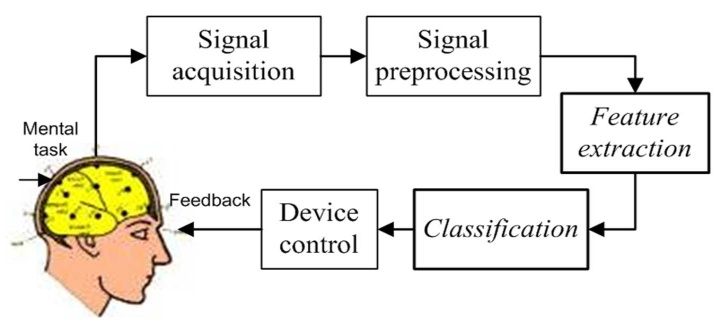
\includegraphics[width=0.9\textwidth]{bci.png}}
	\caption{Общая схема работы нейрокомпьютерных интерфейсов.}
	\label{bci}
	\end{figure}


	\subsection{Предобработка}
	\par Предобработка сигнала проводится с целью удаления артефактов (спонтанные сокращения мышц, моргание и т.п.), а также нейтрализации имеющихся шумовых компонент. Кроме того, зачастую интересующая информация содержится в определённом диапазоне частот, а остальные компоненты являются малоинформативными.
	\begin{itemize}
	\item {\bf Удаление постоянного амплитудного смещения}
	\par {\it Постоянное амплитудное смещение} или {\it DC offset} (англ. {\it direct current offset}, постоянное смещение потока) ~--- отклонение волновой формы относительно оси нулевого уровня сигнала. Амплитудное смещение, наблюдаемое в электроэнцефаллограмме, может быть разложено на две основные составляющие: постоянное смещение, возникающее из-за технических особенностей передачи данных, и  смещение, возникающее из-за взаимодействия электрической цепи с потенциалом тела.
	\item {\bf Полосовая фильтрация}
	\par TODO: написать про фильтры НЧ, ВЧ, полосы
	\par В электроэнцефалограмме здорового человека выделяют несколько характерных составляющих электрических колебаний, называемых ритмами, различающихся частотным диапазоном, а также амплитудой, формой волны и другими характеристиками. Считается, что каждый ритм соответствует некоторому определённому состоянию мозга и связан с определёнными церебральными механизмами. С целью выявления компонент, отвечающих соответствующим ритмам, применяются методы фильтрации в заданном диапазоне частот. Диапазон частот выбирается, исходя из априорной информации о ритмах. К примеру, для выделения компоненты, отвечащей за воображаемые движения различных частей тела, используется диапазон $\mu$-ритма (8--13 Гц).
	\item {\bf Отбор электродов}
	\par Современные электроэнцефалографы оснащены десятками электродов, однако информация, получаемая при помощи такого количества сенсоров, является избыточной. Кроме того, увеличение числа электродов ведёт к повышению стоимости устройства и времени на подготовку к использованию, что является недопустимым для электроэнцефалографов, разработанных для коммерческого использования. В связи с этим в современных исследованиях по тематике нейрокомпьютерных интерфейсов наиболее распространены два подхода к решению данной проблемы:
	\begin{enumerate}
	\item выбор электродов с учётом априорных знаний о локализации компонент сигнала на скальпе;
	\item использование методов отбора признаков.
	\end{enumerate}
	\end{itemize}
	\subsection{Построение признакового пространства}
	\par Применение классических методов распознавания в классе задач нейрокомпьютерных интерфейсов не представляется возможным в силу множества причин, среди которых высокая степень зашумлённости данных, высокая размерность пространства, а также многомерность самих сигналов и т.п. В связи с этим этап построения признакового пространства является самым важным в процессе решения задачи. Проблема заключается в том, что не существует единого метода поиска нового признакового пространства. Каждый исследователь сталкивается с необходимостью поиска признакового пространства для эффективного решения конкретной поставленной задачи с использованием конкретного оборудования. 
	\begin{itemize}
	\item
	{\bf Преобразование Фурье}
	\par TODO: Нужно ли упомянуть теорему Котельникова?
	\par Зачастую анализ сигналова проводится при помощи разложения на "базисные" функции, каждая из которых отвечает некоторой частоте. Таким образом можно проанализировать степень выраженности колебаний некой частоты. В частности, преобразование Фурье использует в качестве базисных функций синусоиды. Для дискретных сигналов, имеющих место в задаче построения нейрокомпьютерного интерфейса, применяется дискретное преобразование Фурье.
	\par Пусть имеется дискретный сигнал $x = (x_0, \dots, x_{N-1})$. Тогда его можно представить в виде линейной комбинации дискретных синусоид следующего вида:
$$x_n = \sum_{k=0}^{\frac{N}{2}} C_k \cos{\frac{2 \pi k (n + \phi_k)}{N}} = \sum_{k=0}^{\frac{N}{2}} A_k \cos{\frac{2 \pi k n}{N}} + \sum_{k=0}^{\frac{N}{2}} B_k \sin{\frac{2 \pi k n}{N}}, n = \overline{0, N-1}.$$
	Для каждого сигнала можно однозначно определить коэффициенты $A_k, B_k,$ называемые {\it спектром} сигнала. Получение коэффициентов при имеющемся сигнале называется {\it прямым преобразованием Фурье}, в то время как обратный процесс, синтез сигнала по имеющимся, коэффициентам называется {\it обратным преобразованием Фурье}. Наиболее часто используется {\it быстрое преобразование Фурье (БПФ)}, позволяющее выполнять преобразования значительно быстрее за счёт  наличия повторяющихся значений при вычислении в силу периодичности функции синуса. 
	\par По аналогии можно произвести подобное разложение и для двумерного сигнала, при этом непосредственное вычисление двумерного ДПФ по полученным формулам требует огромных вычислительных затрат. Однако можно показать, что двумерное ДПФ обладает свойством сепарабельности, то есть его можно вычислить последовательно по двум измерениям. 
	\par Отметим также, что преобразование Фурье является чувствительным к шуму.
	\item
	{\bf Вейвлет-преобразование}
	\par Вейвлет-преобразование — интегральное преобразование, которое представляет собой свертку вейвлет-функции, обладающей рядом характерных свойств, с сигналом. По аналогии с преобразованием Фурье происходит некое разложение исходного сигнала. Для дискретных сигналов используется дискретное вейвлет-преобразование.
	\par Пусть имеется дискретный сигнал $x = (x_0, \dots, x_{N-1})$. Дискретное вейвлет-преобразование применяется путём применения набора фильтров. Сигнал подвергается действию низкочастотного фильтра с импульсным откликом $g$ и высокочастотного фильтра с импульсным откликом $h$, в результате чего получаются коэффициенты аппроксимации и детализирующие коэффициенты соответственно. После этого каждый из наборов коэффициентов прореживается в 2 раза. Кроме того, это разложение можно повторить несколько раз для дальнейшего увеличения частотного разрешения с дальнейшим прореживанием коэффициентов после НЧ и ВЧ-фильтрации. Это можно представить в виде двоичного дерева, где листья и узлы соответствуют пространствам с различной частотно-временной локализацией. Схема действия одно- и трёхуровнего вейвлет-преобраования приведена на рис.~\ref{wavelet_scheme}.

\begin{figure}[H]
\begin{minipage}[H]{1.0\linewidth}
\center{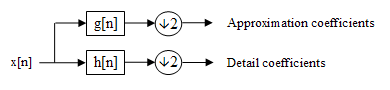
\includegraphics[width=0.5\linewidth]{wave1.png} \\ а)}
\end{minipage}
\begin{minipage}[H]{1.0\linewidth}
\center{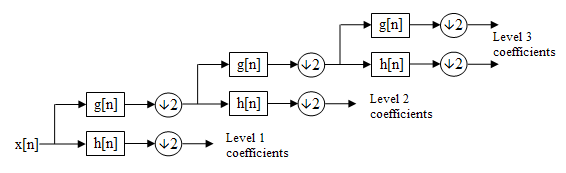
\includegraphics[width=0.5\linewidth]{wave2.png} \\ б)}
\end{minipage}
\caption{Зависимость сигнала от шума для данных.}
\label{wavelet_scheme}
\end{figure}
	\item
	{\bf Метод главных компонент}
	\par Метод главных компонент (англ. Principal Components Analysis, PCA) — один из основных способов уменьшить размерность данных, потеряв наименьшее количество информации. Данный метод производит поиск преобразования данных в семействе линейных функций:
$$x = Wt + \mu = t_1 {\textbf w_1} + \dots + t_d {\textbf w_d} + \mu,$$
где $x \in \mathbb{R}^D, t \in \mathbb{R}^d$ - исходный и преобразованный сигналы соответственно, $W = ( {\textbf w_1}| \dots | { \textbf w_d}) \in \mathbb{R}^{D \times d}, \mu \in \mathbb{R}^D.$ Геометрическим смыслом данного преобразования является проекция данных на гиперплоскость с базисом ${\textbf w_1}, \dots, {\textbf w_d}$. Данный метод предпологает выбор гиперплоскости в соответствии с минимизацией суммы квадратов отклонений исходных объектов от их проекций.
	\par Можно показать, что векторы главных компонент — это ортонормированный набор  $\left\{a_1,..., a_n \right\}$ собственных векторов эмпирической ковариационной матрицы, расположенных в порядке убывания собственных значений $\lambda: \lambda_1 \ge \lambda_2 \ge ... \ge \lambda_n \ge 0$. Большая часть вариации данных будет сосредоточена в первых координатах, что позволяет перейти к пространству меньшей размерности.
	\item
	{\bf Метод независимых компонент}
	\par Метод независимых компонент (англ. Independent Component Analysis) является сравнительно новым методом. Впервые алгоритм был предложен Беллом и Сейновским в 1995. Он 
позволяет восстановить независимые источники, которые линейно смешиваются и регистрируются несколькими датчиками, причём количество источников не должно превосходить количество датчиков для достижения высоких результатов. Кроме того, необходимо, чтобы источники были статистически независимы, а распределение сигнала каждого из источников не было нормальным. Существует несколько различных подходов к решению поставленной задачи, которые отличаются в то числе и используемым определением "независимости" источников. Чаще всего для процесс нахождения независимых компонент осуществляется путём минимизации совместной информации или максимизации отличия распределения от нормального.
	\par Этот метод идеально подходит для анализа ЭЭГ при выделении артефактов глазных движений, а также для анализа вызванных потенциалов при выделении компонент, связанных с различными (независимыми) процессами.
	\item
	{\bf Общий пространственный фильтр}
	\par Общий пространственный фильтр (англ. Common Spatial Pattern Filter, CSP) реализует метод декомпозиции многоканального ЭЭГ сигнала, основанный на обучении по прецедентам.
	\par Рассматривается задача классификации многомерных сигналов на 2 класса. Целью метода является разложение исходного сигнала на аддитивные составляющие таким образом, чтобы максимизировать дисперсию первых компонент и минимизировать дисперсию последених для объектов первого класса и добиться обратной ситуации для объектов второго класса. Матрица декомпозиции может быть найдена в результате одновременной диагонализации выборочных матриц ковариации для каждого из классов. В результате может быть сформирован вектор характерных признаков путём соединения значений некоторого количества первых и последних компонент декомпозированного сигнала.
	\par Метод также может быть обобщён для задачи с количеством классов, больших двух, путём разбиения исходной задачи на бинарные подзадачи с использованием схем <<один против одного>> или <<один против всех>>.
	\item
	{\bf Статический анализ сигнала}
	\par Также зачастую используются вычисленные по фиксируемому сигналу статические характеристики, такие как ... (TODO: перечислить)
	
	\end{itemize}
	\subsection{Классификация}
	\par После построения искомого признакового пространства алгоритм, используемый для классификации преобразованных объектов, играет не столь значительную роль. Наиболее часто в исследованиях по тематике {\it BCI} используются следующие типы классификаторов (TODO: описать плюсы-минусы и общие идеи):
	\begin{itemize}
	\item
	{\bf Байесовский классификатор}
	\par Байесовский классификатор — широкий класс алгоритмов классификации, основанный на принципе максимума апостериорной вероятности. Для классифицируемого объекта вычисляются функции правдоподобия каждого из классов, по ним вычисляются апостериорные вероятности классов. Объект относится к тому классу, для которого апостериорная вероятность максимальна.
	\par Байесовский подход к классификации основан на теореме, утверждающей, что если плотности распределения каждого из классов известны, то искомый алгоритм можно выписать в явном аналитическом виде. Более того, этот алгоритм оптимален, то есть обладает минимальной вероятностью ошибок.
	\par На практике плотности распределения классов, как правило, не известны. Их приходится оценивать (восстанавливать) по обучающей выборке. В результате байесовский алгоритм перестаёт быть оптимальным, так как восстановить плотность по выборке можно только с некоторой погрешностью. Зачастую в исследования по тематике создания нейрокомпьютерного интерфейса в качестве функции правдоподобия для объекта используется смесь нормальных распределений.
	\item
	{\bf Линейный дискриминант Фишера}
	\par Линейный дискриминант Фишера (ЛДФ) -- особый вариант байесовского классификатора. Рассмотрим задачу классификации на два класса. Предполагается, что обучающая выборка составлена таким образом, что классы распределены по нормальному закону, а матрицы ковариаций классов равны. Простота классификации линейным дискриминантом Фишера -- одно из достоинств алгоритма: в случае с двумя классами в двумерном признаковом пространстве разделяющей поверхностью будет прямая. Если классов больше двух, то разделяющая поверхность будет кусочно-лиинейной.
	\par Данный метод классификации не требует больших вычислительных затрат, а потом является распространённым для онлайн-приложений.
	\item
	{\bf Метод опорных векторов}
	\par Метод опорных векторов (англ. SVM, support vector machine) — набор схожих алгоритмов обучения с учителем, принадлежащий к семейству линейных классификаторов. Особым свойством метода опорных векторов является непрерывное уменьшение эмпирической ошибки классификации и увеличение зазора, поэтому метод также известен как метод классификатора с максимальным зазором. Кроме того, на положение разделяющей гиперплоскости в действительности оказывает влияние небольшая часть объектов обучающей выборки. Метод также обобщается на случай нелинейной разделяющей поверхности.
	\par Зачастую используется в исследования по нейрокомпьютерных интерфейсах в силу сводимости к задаче квадратичного программирования и последующей эффективности вычислений.
	\item
	{\bf Метод k ближайших соседей}
	\par Метод k ближайших соседей (англ. k-nearest neighbor algorithm, kNN) — метод автоматической классификации объектов. Основным принципом метода ближайших соседей является то, что объект присваивается тому классу, который является наиболее распространённым среди соседей данного элемента. Соседи выбираются из обучающей выборки, и, исходя из ключевого для данного метода значения k, высчитывается, какой класс наиболее многочислен среди них.
	\par Таким образом, если в процессе формирования признакового пространства удалось некоторым образом локализовать объекты каждого из классов в некоторой области пространства, данный метод может быть использован для классификации преобразованных объектов. Кроме того, среди достоинств данного метода ледует упомянуть вычислительную простоту, что делает его простым для использования в онлайн-приложениях.
	\end{itemize}

\newpage

\section{Проведение эксперимента?}
	\subsection{Используемое оборудование}
	\quad\,\,\, Несмотря на то что существует множество различных методов фиксации активности головного мозга (электрокортикограмма, электроокулограмма и др.), в настоящее время основным способом получения сигнала головного мозга является электроэнцефалограмма. 
	\par {\it Электроэнцефалография (ЭЭГ)} — раздел электрофизиологии, изучающий закономерности суммарной электрической активности мозга, отводимой с поверхности кожи головы или мозга, а также метод записи таких потенциалов. Получение электроэнцефалограммы осуществляется с помощью электроэнцефалографа. Существуют различные устройства для записи ЭЭГ, отличающиеся следующими характеристиками: 
	\begin{itemize}\itemsep0pt
	\item
	характеристики принимающего сигнала (частота, количество шума в сигнале);
	\item
	инвазивность (степень имплантирования электродов в кору головного мозга);
	\item
	количество электродов;
	\item
	покрываемая площадь (среднее количество влияющих на сигнал нейронов, снимаемых одним электродом).
	\end{itemize}
	\par По инвазивности устройства делятся на {\it погружные}, {\it частично-погружные} и {\it непогружные} в зависимости от расположения электродов (электроды вживлены в мозг/сращены с нервами, находятся на поверхности мозга/рядом с нервами или находятся на поверхности кожи головы соответственно).

	\par Устройства с непогружным интерфейсом делятся на {\it мокрые} и {\it сухие} в зависимости от того, необходимо ли смачивание электродов проводящей жидкостью для осуществления контакта.
	\par По типу электродов устройства делятся на {\it пассивные} и {\it активные} в зависимости от того, проивзодится ли после снятия электродом сигнала его первичная обработка.

	
	\par В настоящей работе для записи электроэнцефалограммы использовалось устройство {\it Emotiv EPOC}. Это устройство было разработано австралийской компанией {\it Emotiv Systems}, основанной в 2003 году. Данная компания входит в число трёх основных участников рынка потребительских устройств BCI наряду с компаниями {\it NeuroSky} и {\it OCZ}, однако {\it Emotiv EPOC} имеет значительно большее число электродов, чем устройства компаний-конкурентов, и незначительно более высокую стоимость. 
	\par Общий вид устройства изображён на рис.~\ref{Emotiv}, устройство обладает следующими характеристиками:
	\begin{itemize}\itemsep0pt
	\item
	число датчиков — 14;
	\item
	тип датчиков — пассивные, мокрые;
	\item
	частота дискретизации — 128 Гц;
	\item
	способ связи — беспроводная радиосвязь;
	\item
	гироскопы — 2 шт.;
	\item
	инвазивность — непогружной.
	\end{itemize}

	\begin{figure}[H]
	\center{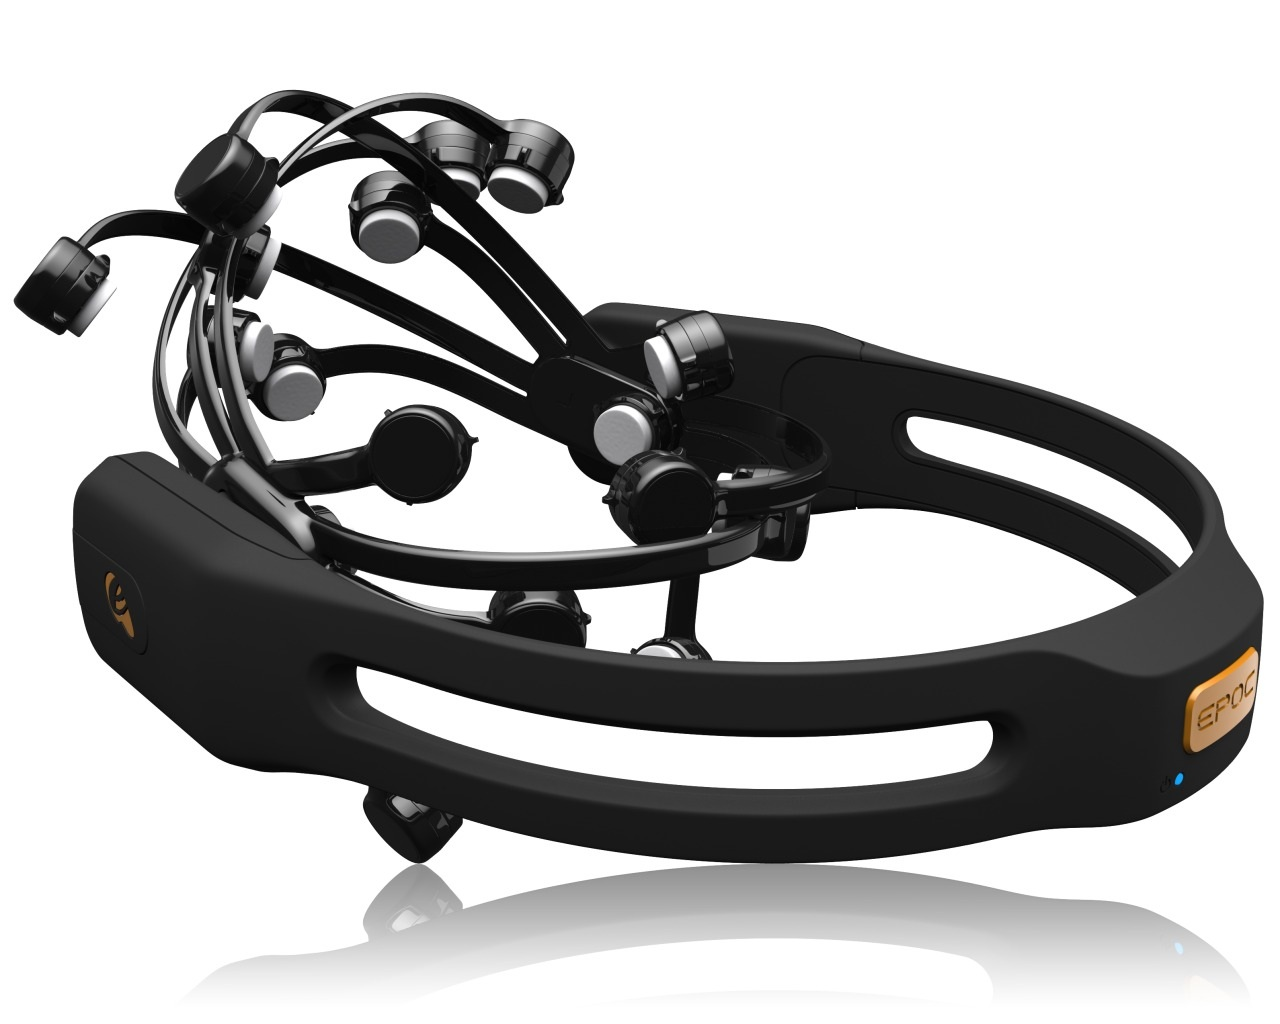
\includegraphics[width=0.9\textwidth]{Emotiv.jpg}}
	\caption{{\it Emotiv EPOC} ~--- устройство, используемое для записи данных.}
	\label{Emotiv}
	\end{figure}

	\par Расположение электродов согласно международной системе размещения электродов <<10 -- 20>> изображено на рис.~\ref{electrode_map}.
	\par Устройство {\it Emotiv EPOC} было использовано в силу своей доступности. Также достоинствами данного устройства являются портативность, простота использования и небольшие размеры. В то же время оно обладает и рядом недостатков: низкая точность снимаемого сигнала и ненадёжная фиксация устройства на голове человека. В рамках настоящей работы будет предпринята попытка купировать недостатки устройства применяемыми методами обработки и классификации сигнала.

	\begin{figure}[H]
	\center{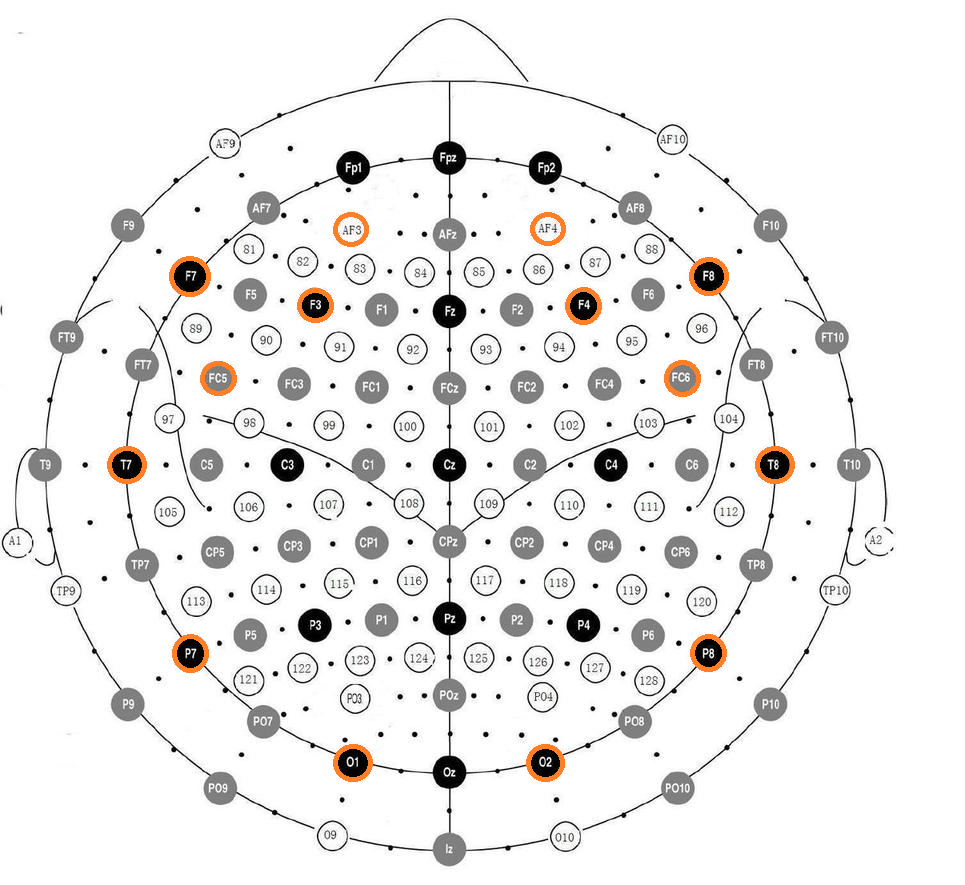
\includegraphics[width=0.9\textwidth]{electrode_map_1020.png}}
		\caption{Расположение электродов на голове человека согласно международной системе размещения электродов <<10--20>>. Электроды устройства {\it Emotiv EPOC} выделены оранжевым цветом.}
	\label{electrode_map}
	\end{figure}

%	\par TODO: Нужен ли отдельный раздел для Хиперы? Если да, то как назвать этот раздел и раздел про Хиперу?
%	\par В качестве динамического объекта, приводимого в движение при помощи ментальных команд, было использовано устройство {\it Khepera II}. Данное устройство было разработано швейцарской компанией {\it K-team Corporation}.
%	\par Устройство оснащено двумя моторами, приводящими в движение колёса по бокам робота. Устройство управляется путём осуществления команд установки либо изменения скоростей вращения каждого из моторов. (TODO: Нужно ли писать детали о том, как подключается робот к компьютеру, какими командами управляется и т.д.?) Таким образом, имеется возможность осуществления прямолинейного движения либо поворота устройства в плоскости его движения, тем самым команды поворота по и против часовой стрелке на фиксированный угол относительно текущей траектории позволяют управлять движением устройства на плоскости без остановки. Если же, помимо того, использовать команды начала движения и остановки устройства, появится возможность полного управления устройством при движении на плоскости.

\subsection{Парадигма эксперимента}
	\par Как правило, в исследованиях на основе визуальных стимулов используется следующая схема получения данных:
	\begin{itemize}
	\item
	Испытуемому в течение $t_1$ секунд демонстрируется визуальный стимул либо ментальное задание, которое предстоит выполнить. 
	\item
	В течение $t_2$ секунд испытуемый сосредотачивает внимание на визуальном стимуле либо выполняет указанное ментальное задание. Кроме того, в процессе этого действия происходит запись данных.
	\item Визуальный стимул перестаёт демонстрироваться испытуемому, проводится краткая пауза для восстановления расслабленного состояния и подготовки к следующей итерации.
	\end{itemize}

	\par После изучения материалов по исследуемой тематике и различных видов парадигм, используемых для проверки надёжности систем управления с использованием нейрокомпьютерных интерфейсов в различных приложениях было принято решение два типа парадигм, близких к предложенным в (Пиччоне) с использованием двух различных видов визуальных стимулов. ...
	\par Поулчение данных производилось следующим образом. Испытуемый располагался лицом к монитору компьютера с устройством {\it Emotiv EPOC}, расположенным на голове. На экране монитора было изображено квадратное поле, разбитое на 100 равных квадратов прямыми, параллельными его сторонам, путём деления каждой стороны на 10 отрезков. Каждый из квадратов являеся возможным положением курсора на экране компьютера. Целью испытуемого являлось управление курсором в виде голубого квадрата, расположенного на экране компьютера от начального до обозначенного конечного положения. Четыре визуальных стимула выделялись на экране последовательно случайным образом, в каждый момент времени было выделено не более одного визуаильного стимула. Каждый из стимулов соответствовал одному из возможных направлений движения курсора (вверх, вниз, влево, вправо). Испытуемый должен был сконцентрировать внимание на стимуле, отвечающем желаемому направлению движения (т.н. целевой стимул), и игнорировать остальные стимулы, отвечающие нежелательным направлениям движения курсора (т.н. отвлекающие стимулы).
	\par Назовём {\it пробой} последовательность из выделения некоторого визуального стимула в течение 250 мс, а также последующие 1250 мс, необходимые для обработки, классификации данных, генерации и выполнения перемещения курсора. Интервал между двумя выделениями стимулов был установлен равным 2.5 с, включая время, необходимое на обработку и классификацию данных. Назовём {\it сессией} последовательность проб, предпринятых для достижения курсором целевого положения.
	\par Запись ЭЭГ осуществлялась с частотой дискретизации 128 Гц (с внутренней частотой дискретизации устройства 2048 Гц и последующей первичной обработкой) при помощи устройства {\it Emotiv EPOC}. При записи данных устройство находилось в двух различных положениях: положение по умолчанию и инверсированное положение. В положении по умолчанию были использованы данные 10 сенсоров, указанных на рис.~\ref{default} (F3, FC5, T7, P7, O1, O2, P8, T8, FC6, and F4), поскольку данное подмножество обеспечивает покрытие части скальпа, отвечающей за P300-волны. В инверсированном положении были использованы данные 8 сенсоров, указанных на рис.~\ref{reversed}, поскольку они покрывают центральную часть скальпа, которая считается областью, наиболее активно отвечающей за генерацию P300-волн.

\subsection{Схема эксперимента}
	\par 

\newpage
\section{Новые подходы и результаты}

Название этого раздела обязательно надо заменить на~содержательное. 
В~этом разделе, как правило, много подразделов. 

В~дипломной работе не~стоит делать более двух уровней,
достаточно разделов и~подразделов.
Будете писать диссертацию или монографию~--- сделаете три уровня. 
  
\section{Вычислительные эксперименты}

Цель данного раздела:
продемонстрировать, что предложенная теория работает на практике;
показать границы её применимости;
рассказать о~новых экспериментальных фактах.

Чисто теоретические работы могут вообще не~содержать раздела экспериментов
(не~работает, ну и~не~надо~--- зато теория красивая).
Кстати, теоретики имеют право не~догадываться, где, кому и~когда их теории пригодятся.

\subsection{Исходные данные и~условия эксперимента}
Описывается прикладная задача, параметры анализируемых данных 
(например, сколько объектов, сколько признаков, каких они типов), 
параметры эксперимента 
(например, как производился скользящий контроль). 

\subsection{Результаты эксперимента}
Результаты экспериментов представляются в~виде таблиц и~графиков. 
Объясняется точный смысл всех обозначений на графиках, строк и~столбцов в~таблицах. 

\subsection{Обсуждение и~выводы}
Приводятся выводы: 
в~какой степени результаты экспериментов согласуются с~теорией? 
Достигнут ли желаемый результат? 
Обнаружены ли какие-либо факты, не~нашедшие объяснения, и~которые нельзя списать на «грязный» эксперимент?

Обсуждаются основные отличия предложенных методов от известных ранее. 
В~чем их преимущества? 
Каковы границы их применимости? 
Какие проблемы удалось решить, а~какие остались открытыми? 
Какие возникли новые постановки задач?

\section{Заключение}

В~квалификационных работах последний раздел нужен для того, чтобы 
конспективно перечислить основные результаты, полученные лично автором. 

Результатами, в~частности, являются:
\begin{itemize}
\item 
    Предложен новый подход к\dots
\item 
    Разработан новый метод\dots, позволяющий\dots
\item 
    Доказан ряд теорем, подтверждающих (опровергающих), что\dots
\item 
    Проведены вычислительные эксперименты\dots,
    которые подтвердили / опровергли / привели к~новым постановкам задач.
\end{itemize}
    
Цель данного раздела: доказать квалификацию автора. 
Даже беглого взгляда на заключение должно быть достаточно, чтобы стало ясно: 
автору удалось решить актуальную, трудную, ранее не~решённую задачу, 
предложенные автором решения обоснованы и~проверены.

Иногда в~Заключении приводится список направлений дальнейших исследований.

\newpage
Список литературы необходим в~любой научной публикации. 
В дипломной работе он~обязателен. 
Дурным тоном считается:
ссылаться на работы только одного-двух авторов (например, себя или шефа);
ссылаться на слишком малое число работ;
ссылаться только на очень старые работы;
ссылаться на работы, которых автор ни разу не видел;
ссылаться на~работы, которые не~упоминаются в~тексте
или которые не~имеют отношения к~данному тексту.



\end{document}
